

\فصل{راهنمای نصب برنامک}

در این قـسمت راهـنماي نـصب بـرنـامک آورده شـده اسـت. این مـراحـل بـراي سیستم عـامـل انـدروید فـرض شـده اسـت. بـراي نـصب بـرنـامک روي سیستم عـامـل آي‌اواس نیاز بـه حـساب بـرنـامـه نـویس اپـل و انتشار آن در فروشگاه برنامک آن داریم که هزینه سالانه ۱۰۰ دلاري دربردارد.
\newline
بـرنـامک انـدرویدي را میتـوانید از آدرس پیوند https://github.com/mahdihs76/drugdetector releases/tag/v1.0 بارگیري کنید. این برنامک روي نسخه اندروید ۱.۴ و بالاتر قابل نصب است.
\newline
\شروع{شکل}[ht]
\begin{center}
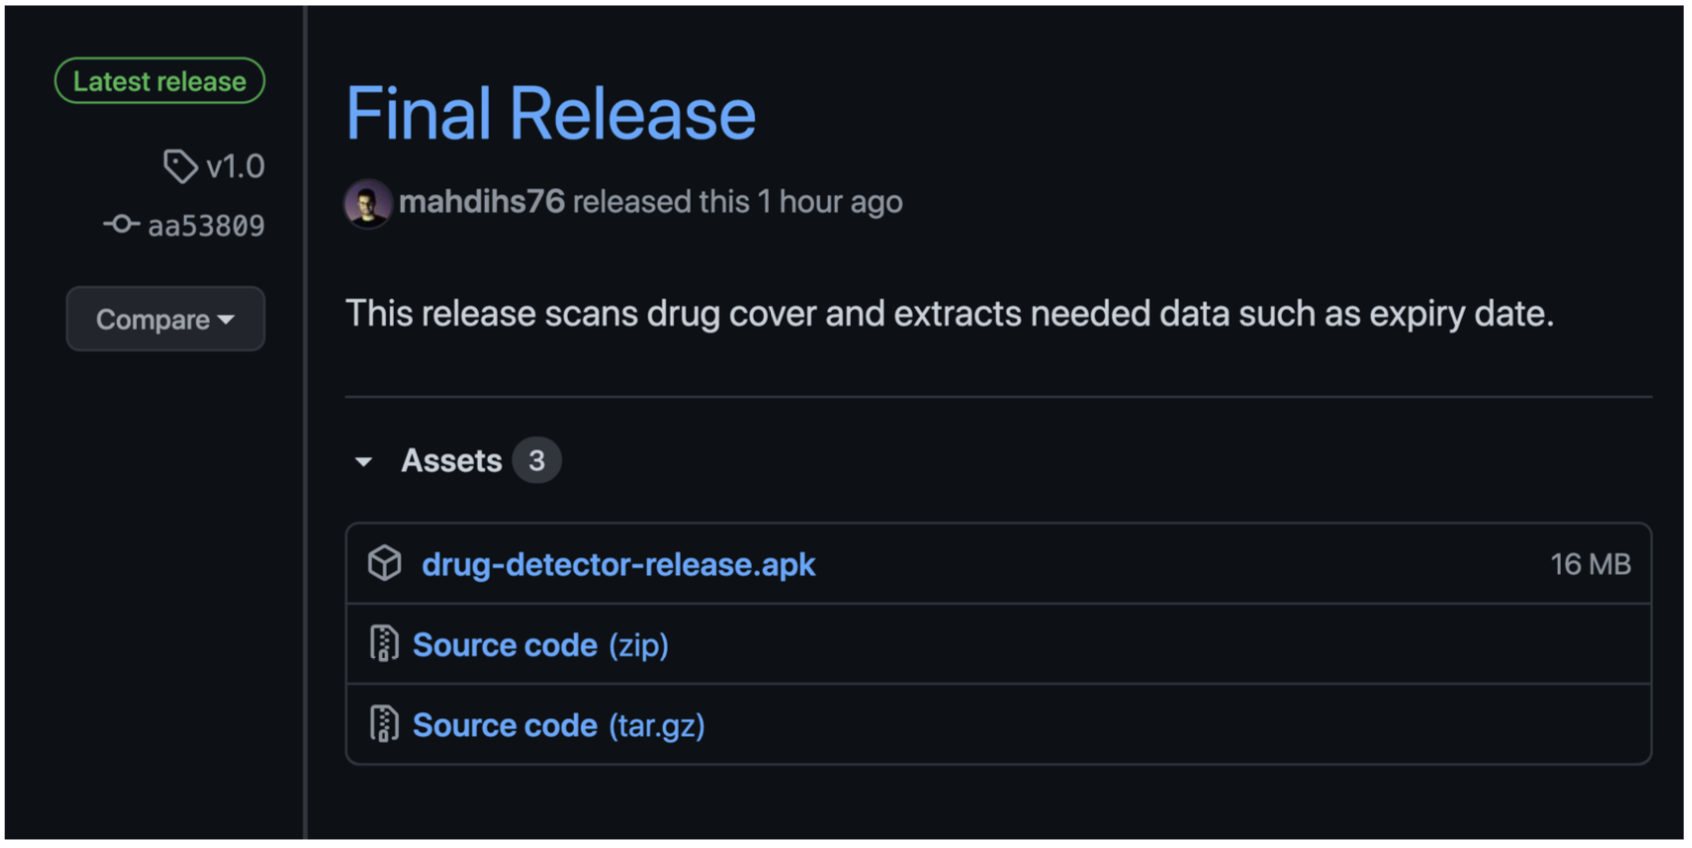
\includegraphics[scale=0.5]{front/template/images/release.png}
\end{center}
\شرح{نسخه 1.0.0 منتشر شده برنامک در گیت‌هاب }
\پایان{شکل}


\فصل{آزمون کیفیت برنامک}

عملکرد این برنامک بر روی یک مجموعه داده دریافت شده از داروخانه هدف بررسی شد و دقت مناسبی در تشخیص درست اطلاعات جعبه دارو به همراه داشت. در ادامه نمایی از عملکرد برنامک بر روی داروی Rozaprazole نمایش داده شده است.
\newline
\شروع{شکل}[ht]
\begin{center}
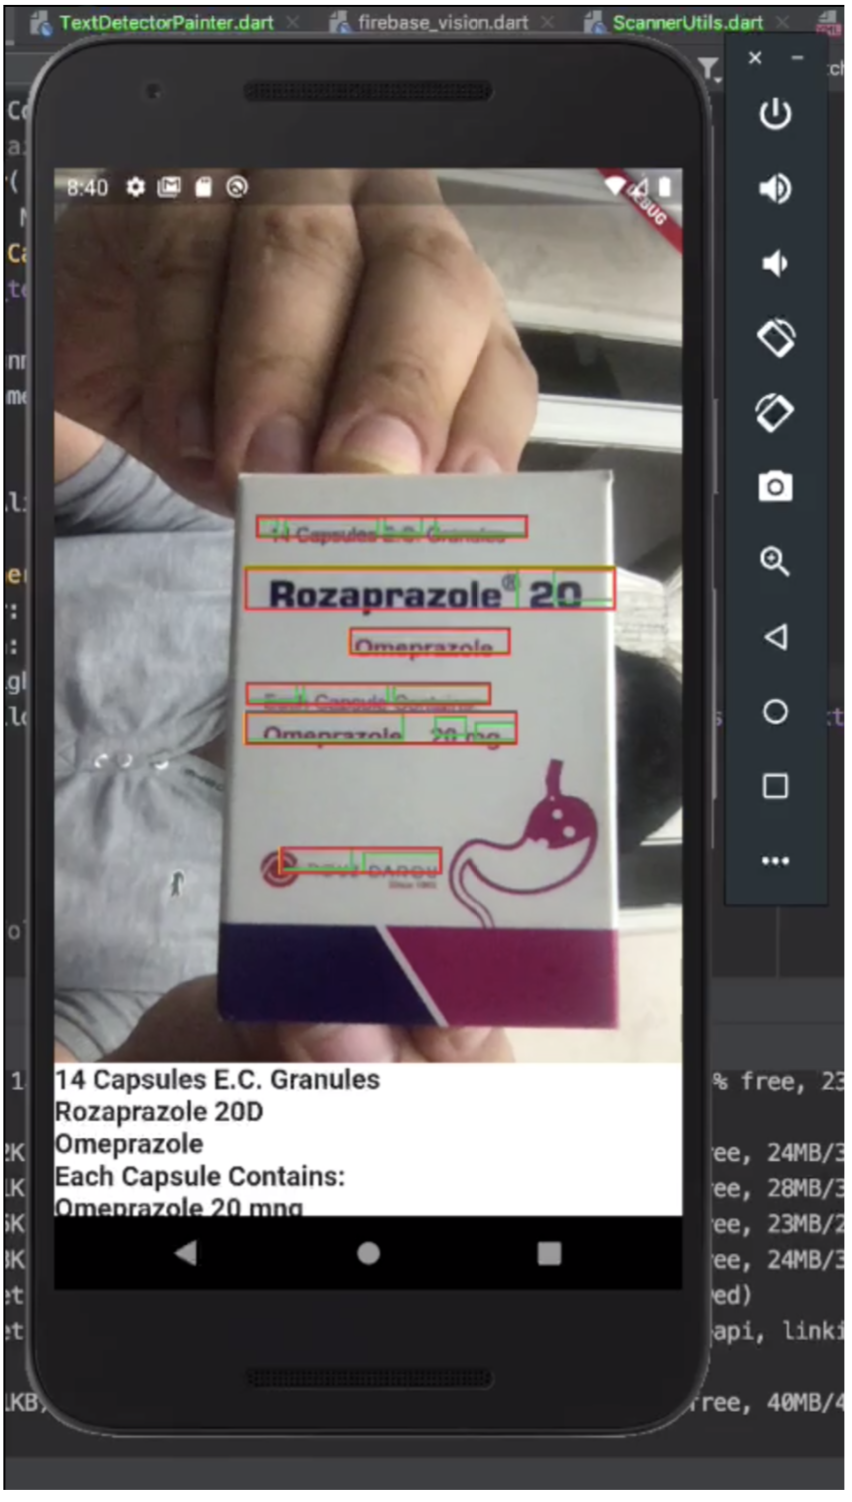
\includegraphics[scale=0.7]{front/template/images/test.png}
\end{center}
\شرح{استخراج اطلاعات داروی Rozaprazole }
\پایان{شکل}

